\documentclass[11pt,a4paper]{article}

\usepackage[margin=2.5cm]{geometry}
\usepackage[T1]{fontenc}
\usepackage[utf8]{inputenc}
\usepackage{lmodern}
\usepackage{microtype}
\usepackage{graphicx}
\usepackage{booktabs}
\usepackage{tabularx}
\usepackage{array}
\usepackage{amsmath}
\usepackage{siunitx}
\usepackage{xcolor}
\usepackage{caption}
\usepackage{subcaption}
\usepackage{placeins}
\usepackage{natbib}
\usepackage[hidelinks]{hyperref}

\graphicspath{{figures/}}
\setlength{\parindent}{0pt}
\setlength{\parskip}{0.65em}
\renewcommand{\arraystretch}{1.15}
\captionsetup{font=small,labelfont=bf}

\newcommand{\Fa}{\textit{F. aquilonia}}
\newcommand{\Fp}{\textit{F. polyctena}}
\newcommand{\FST}{\ensuremath{F_{ST}}}
\newcommand{\rST}{\ensuremath{r_{ST}}}
\newcommand{\pending}[1]{\textcolor{red}{\textbf{[PENDING: #1]}}}

\title{Supplementary methods and results for locus-specific ancestry sorting:\\ high differentiation without correspondingly high linkage disequilibrium}
\author{}
\date{}

\begin{document}
\maketitle

This document describes the analyses in \texttt{module\_allele\_specific\_sorting}. They ask whether the strong differentiation among the 20 hybrid populations at ancestry-informative loci is accompanied by correspondingly strong linkage disequilibrium (LD), and whether directionally sorted loci share their sorting with nearby markers more than equally differentiated unsorted loci do. Only empirical analyses are included; comparisons with the neutral demographic simulations are deferred until the simulations have been rerun with corrected founder frequencies. Without those comparisons, the results establish an empirical pattern, not its cause. Like the companion BayPass document, the text can be used directly or revised; its main purpose is to support decisions about what to include in the manuscript.

All numbers in the tables are generated from the module's saved outputs by \texttt{R/05\_doc\_tables.R}. Text marked \pending{\ldots} depends on analyses that have not been run.

\tableofcontents
\clearpage

\section{Summary for the main text}
Ancestry-informative regions were strongly differentiated among the 20 hybrid populations, but distant regions usually differentiated different populations. Similarity in ancestry patterns declined rapidly with genetic distance and was close to its background level beyond about 5~cM and between chromosomes. Strong genome-wide differentiation therefore does not reflect a single ancestry pattern repeated across loci (Figure~\ref{fig:decay}).

Sorted loci also showed no greater ancestry-profile similarity or within-population LD with neighbouring markers than matched unsorted loci. This result held for both LD-reduced regions and all unpruned SNPs, including SNPs within each focal locus's own LD cluster. Sorted loci were therefore not embedded in longer ancestry blocks than equally differentiated unsorted loci in comparable recombination contexts. Twenty-five sorted loci in unusually large or otherwise poorly matched LD blocks could not be assessed and remain possible exceptions (Figure~\ref{fig:neighbourhood}; Table~\ref{tab:unmatched}).

Together, the results are consistent with ancestry sorting occurring largely region by region. Comparisons with corrected neutral simulations are still needed before attributing this pattern specifically to selection.


\clearpage
\section{Supplementary methods}
\subsection{Rationale}

A locus is strongly differentiated when its allele frequency varies among populations. Two loci show among-population LD only when their frequencies vary across the \emph{same} populations in a consistent direction. Strong differentiation can therefore accumulate across the genome without strong multilocus LD if ancestry has sorted differently among loci. We refer to this as locus-specific ancestry sorting.

\subsection{Units, populations and orientation}

We analysed 165 individuals from 20 hybrid populations. The distance analysis used 20,807 LD-reduced units representing 51,612 ancestry-informative SNPs (parental diagnostic index $>-25$; hybrids-only LD clustering with a decay-relative quality gate $\rho=0.5$ and a 5~cM merge cap). Combining correlated SNPs avoids counting one genomic region repeatedly but removes some short-range LD, so the neighbourhood analysis was repeated with all 51,612 unpruned SNPs. Genotypes were oriented so that dosage counts the \Fa\ allele, identified from the parental reference samples. For each marker we calculated its \Fa-allele frequency in every population and estimated differentiation among populations using the \citet{weir1984estimating} \FST. Using the project-wide sorting criteria (near-fixation $\phi=0.85$, sorting threshold $\tau=0.6$, binomial $\alpha=0.05$), 1,215 units were sorted toward \Fa\ and 365 toward \Fp.

\subsection{Pairwise statistics}

\paragraph{Ancestry-profile similarity.} For each pair of markers $i$ and $j$, ancestry-profile similarity $c_{ij}$ is the correlation of their oriented allele-frequency profiles across the 20 populations. A positive value means that the same populations were enriched for \Fa\ ancestry at both loci. We repeated the calculation after removing each population's genome-wide ancestry, estimated from all other chromosomes.

\paragraph{Among-population LD and its differentiation ceiling.} Following the decomposition of LD in subdivided populations by \citet{ohta1982linkage}, the among-population component of LD between two loci, normalised as a correlation, is
\begin{equation}
r_{ST,ij}=\frac{\operatorname{cov}_k(F_{ik},F_{jk})}{\sqrt{\bar F_i(1-\bar F_i)\,\bar F_j(1-\bar F_j)}}=c_{ij}\sqrt{G_iG_j},
\qquad G_i=\frac{\operatorname{var}_k(F_{ik})}{\bar F_i(1-\bar F_i)},
\label{eq:rst}
\end{equation}
where $G_i$ is the among-population differentiation of locus $i$ (an unweighted, Nei-type measure computed from population frequencies, distinct from the Weir--Cockerham \FST\ used elsewhere). The product $G_iG_j$ is the \emph{ceiling}: the maximum $r_{ST,ij}^2$, reached if the two loci differentiate the same populations perfectly ($|c_{ij}|=1$). We summarised the \emph{realised fraction} of the ceiling as $\sum r_{ST}^2/\sum G_iG_j$.

\paragraph{Permutation baseline.} With only 20 populations, unrelated profiles still have a non-zero expected squared correlation ($1/19$). We estimated the baseline for each distance class by independently permuting population labels for every unit 500 times. This preserved each unit's allele-frequency profile and differentiation while removing correspondence between loci.

\paragraph{Within-population LD.} We correlated oriented genotypes after centring them within populations and removing variation associated with each individual's genome-wide ancestry, estimated from all other chromosomes. Missing genotypes (2.7\%) were set to the population mean. Because sorted loci are near-fixed in many populations, comparisons of sorted and unsorted loci included only populations in which both markers segregated ($r_w^{\mathrm{poly}}$).

\subsection{Distance analysis}

We evaluated all 9.6 million within-chromosome pairs of LD-reduced units and all 206.8 million cross-chromosome pairs. Pairs were grouped by genetic distance, with physical distance used as a sensitivity analysis; cross-chromosome pairs formed an ``unlinked'' class. Confidence intervals came from 2,000 chromosome-block bootstrap replicates.

\subsection{Neighbourhoods of sorted loci}

If sorting involved long haplotypes, markers near sorted loci should show more similar ancestry patterns and stronger within-population LD than markers near comparable unsorted loci. We matched each sorted locus to up to five unsorted controls based on \FST, local recombination rate, parental allele-frequency difference and local density of LD units (units within $\pm100$~kb). A 1-SD caliper retained 1,552 of 1,577 eligible sorted loci and achieved good balance on all covariates (absolute standardised mean differences $\leq0.04$); narrower calipers excluded many large sorted blocks without improving balance. The 25 unmatched loci are listed separately (Table~\ref{tab:unmatched}).

For each focal locus, we averaged ancestry-profile similarity and $r_w^{\mathrm{poly}}$ with neighbouring markers up to 2~Mb away. We did this both for other LD-reduced units and for all unpruned SNPs, including SNPs in the focal locus's own LD cluster. We also compared the number of SNPs and physical span of the focal LD units. Each sorted locus was compared with the mean of its own controls, and 2,000 chromosome-block bootstrap replicates kept these matched sets intact.


\clearpage
\section{Supplementary results}
\subsection{High differentiation, but among-population LD only over linkage distances}

Ancestry-informative units were strongly differentiated among the hybrid populations (median \FST\ $=0.25$; mean Nei-type $G=0.30$). Consequently, the among-population LD that pairs of units could show if they partitioned the populations identically --- the ceiling $G_iG_j$ in Equation~\eqref{eq:rst} --- was high, $\approx0.091$, and, as expected because it depends only on the loci's marginal differentiation, constant from the closest pairs to pairs on different chromosomes (Table~\ref{tab:decay}; Figure~\ref{fig:decay}a).

Observed among-population LD was a small and rapidly decaying fraction of this ceiling. The realised fraction was 0.243 [95\% CI 0.239, 0.247] for pairs within 5~kb, 0.115 at 5--20~kb and 0.073 at 20--100~kb, and approached the chance level of $1/19=0.053$ beyond $\approx100$~kb (0.058 at 0.5--2~Mb and 0.057 for unlinked pairs; Figure~\ref{fig:decay}b). Among-population LD itself fell from 0.022 to 0.005, a fourfold decline, while the ceiling did not change. Residualised concordance showed the same pattern: 0.387 within 5~kb, 0.068 at 20--100~kb, 0.005 at 0.5--2~Mb and $-0.0004$ [$-0.0007$, $0.0000$] for unlinked pairs. Raw concordance between unlinked units (0.033) was slightly positive, reflecting the shared gradient in genome-wide ancestry among populations that residualisation removes.

The same pattern held in every \FST\ class (Figure~\ref{fig:decay-fst}). Pairs of highly differentiated units had the highest ceiling (0.147) and also realised a somewhat larger fraction of it at short range (0.297 within 5~kb, versus 0.206 for the least differentiated tertile), consistent with the weak positive relationship between \FST\ and local concordance reported in the population-partitioning analyses. For unlinked pairs, however, the realised fraction was at chance level in all classes (0.057--0.059), so that the most differentiated loci in the genome showed no more among-population LD with each other than expected from 20 populations alone.

Within-population LD decayed in parallel, from $r_w^2=0.183$ within 5~kb to 0.030 at 20--100~kb and to a background of 0.008 beyond 2~Mb, equal to the value for unlinked pairs. Adjusting for individual hybrid index changed none of these values in the third decimal place: admixture LD generated by among-individual variation in overall ancestry is negligible within these populations.

On the genetic-map scale (Figure~\ref{fig:decay-cm}), concordance and LD were still above background at 1--5~cM and reached it only beyond 5~cM. The realised fraction was lower for pairs less than 0.001~cM apart (0.153) than for pairs 0.001--0.01~cM apart (0.217). Pairs in the first class include physically distant markers within recombination cold spots, so this non-monotonicity probably reflects heterogeneity among cold-spot regions rather than a simple distance effect; it has not been examined further.

Together, these results show how the ancestry-informative genome can be broadly and strongly differentiated while carrying among-population LD only where loci are physically linked: differentiation accumulates locus by locus, but different loci, beyond the scale of linkage, distinguish different subsets of populations.

\begin{figure}[htbp]
  \centering
  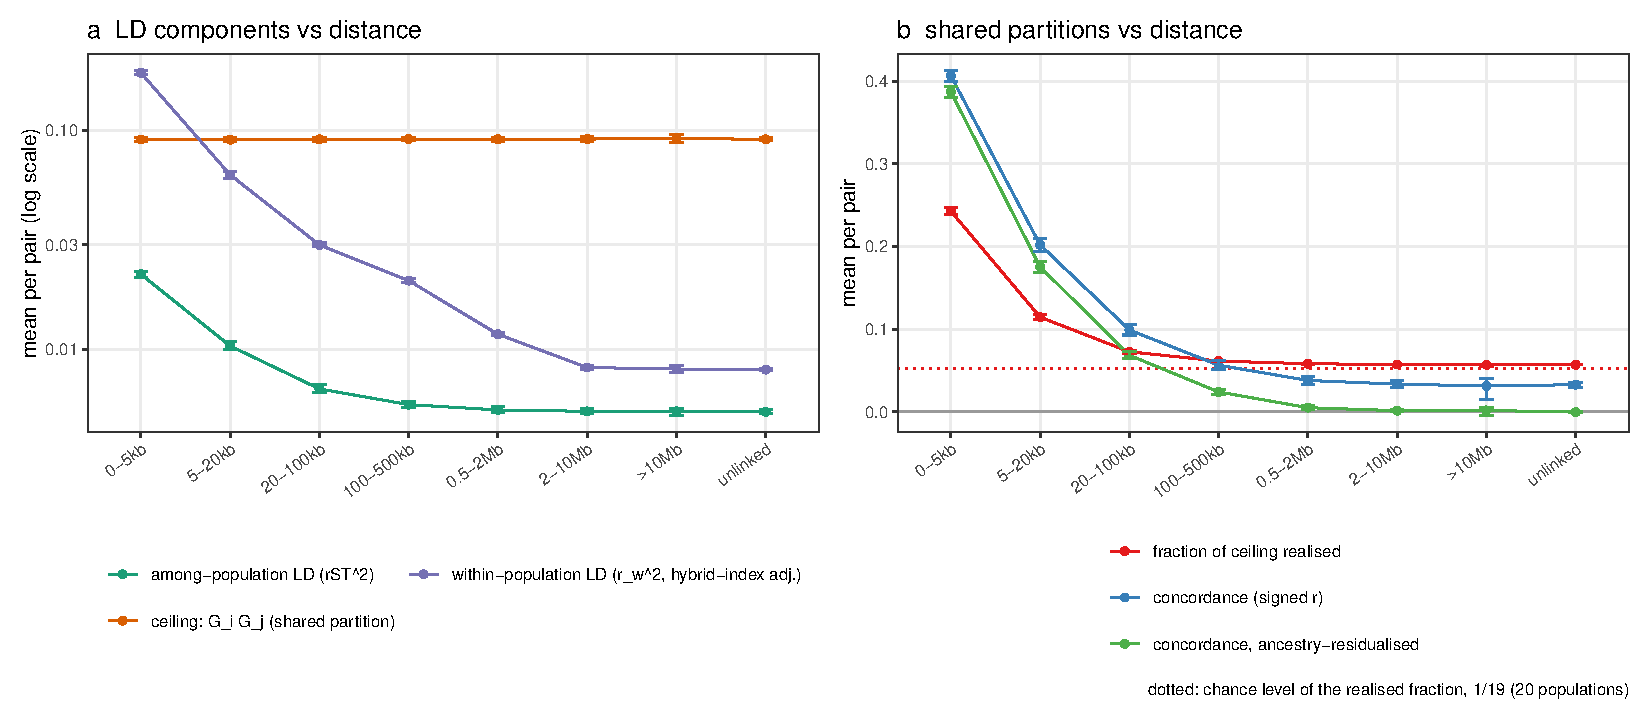
\includegraphics[width=\textwidth]{02_fst_vs_ld_decay.pdf}
  \caption{\FST\ versus LD along a distance axis. \textbf{a}, Means per pair (log scale) of the among-population LD ceiling $G_iG_j$ (the among-population LD two loci with their observed differentiation would show if they partitioned the populations identically), the observed among-population LD $r_{ST}^2$, and within-population LD $r_w^2$ adjusted for individual hybrid index. \textbf{b}, Fraction of the ceiling realised ($\sum r_{ST}^2/\sum G_iG_j$; dotted line: chance level 1/19 for 20 populations), and raw and ancestry-residualised concordance. Unlinked: all 206.8 million cross-chromosome pairs. Error bars: 95\% chromosome-block bootstrap intervals.}
  \label{fig:decay}
\end{figure}

\begin{figure}[htbp]
  \centering
  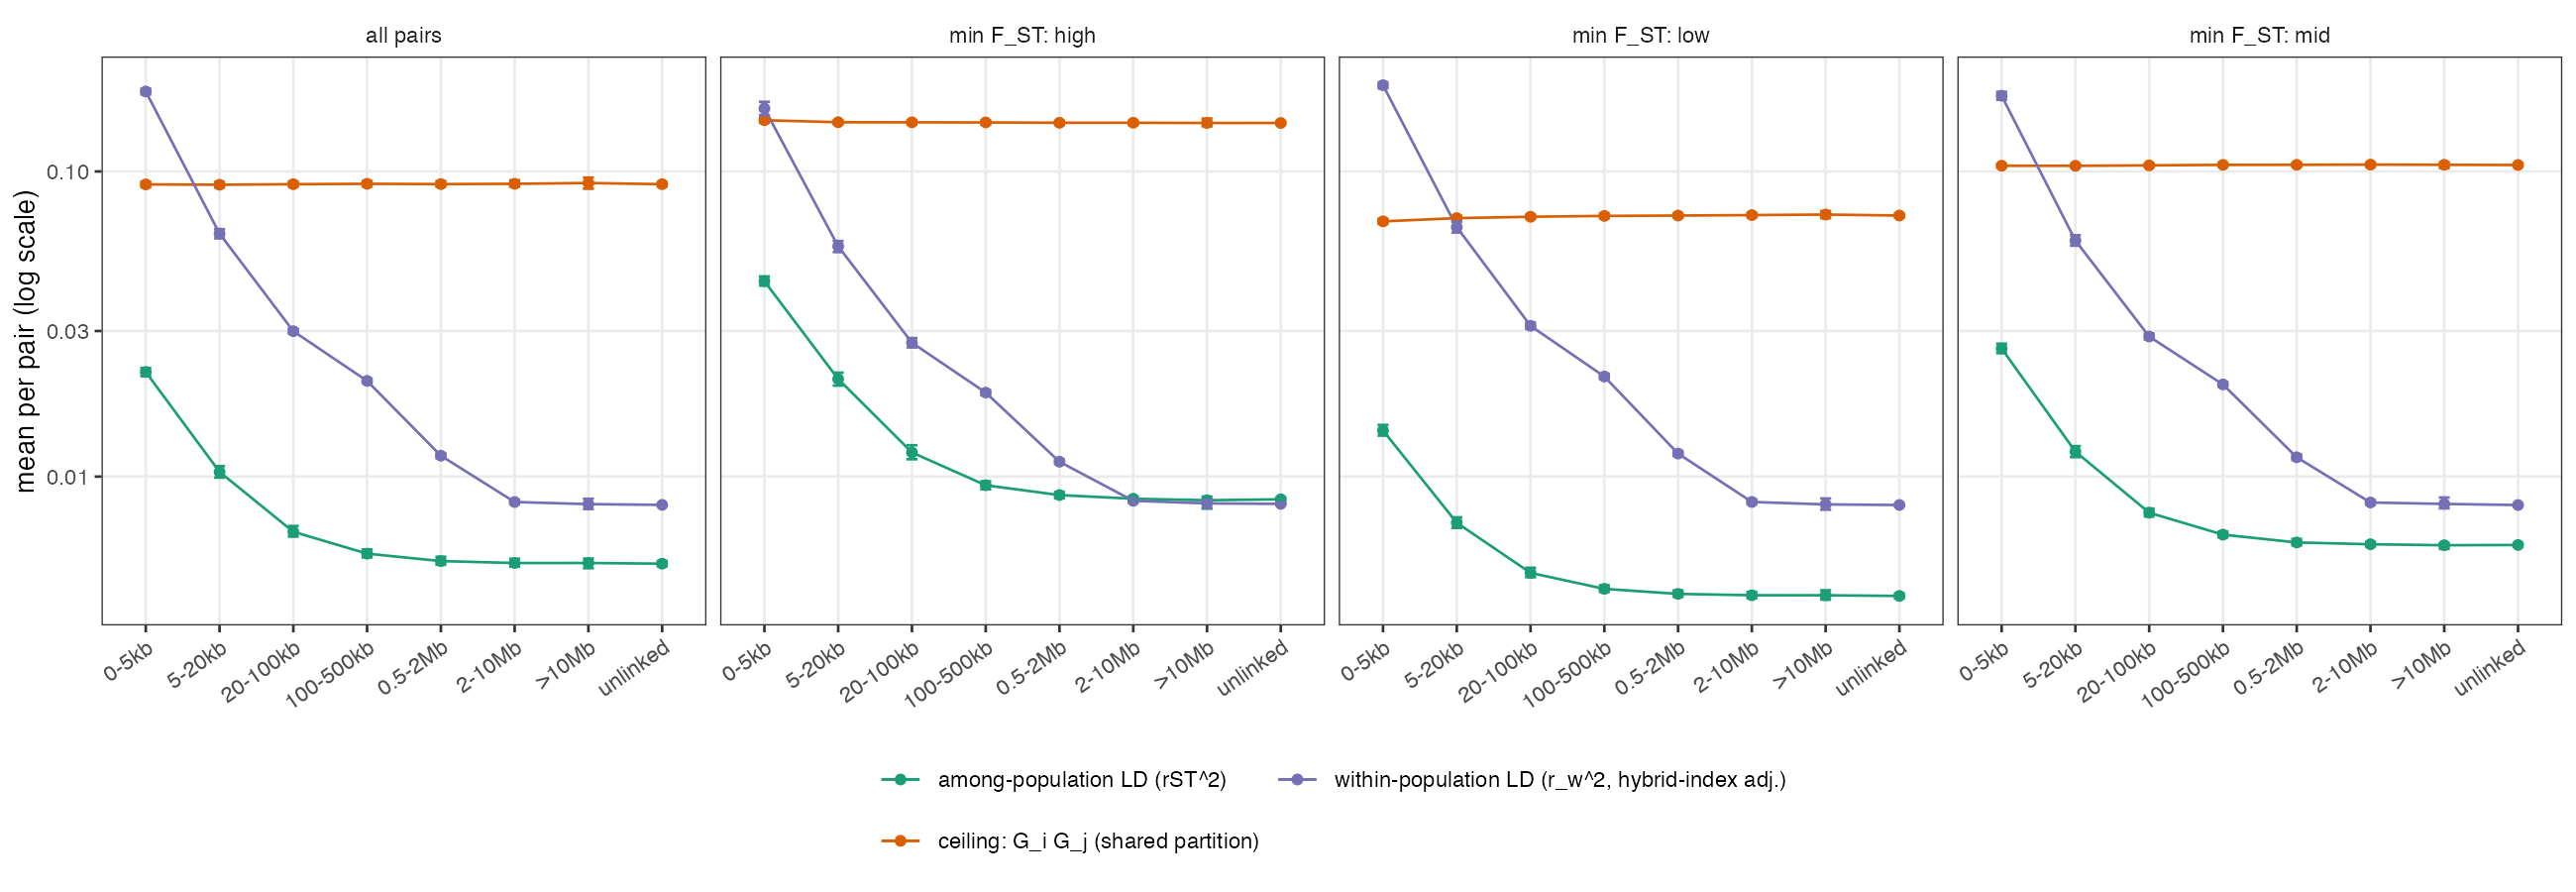
\includegraphics[width=\textwidth]{02_fst_vs_ld_decay_by_fst_class.png}
  \caption{As Figure~\ref{fig:decay}a, stratified by the smaller \FST\ of the two units in a pair (tertiles of unit \FST).}
  \label{fig:decay-fst}
\end{figure}

\begin{figure}[htbp]
  \centering
  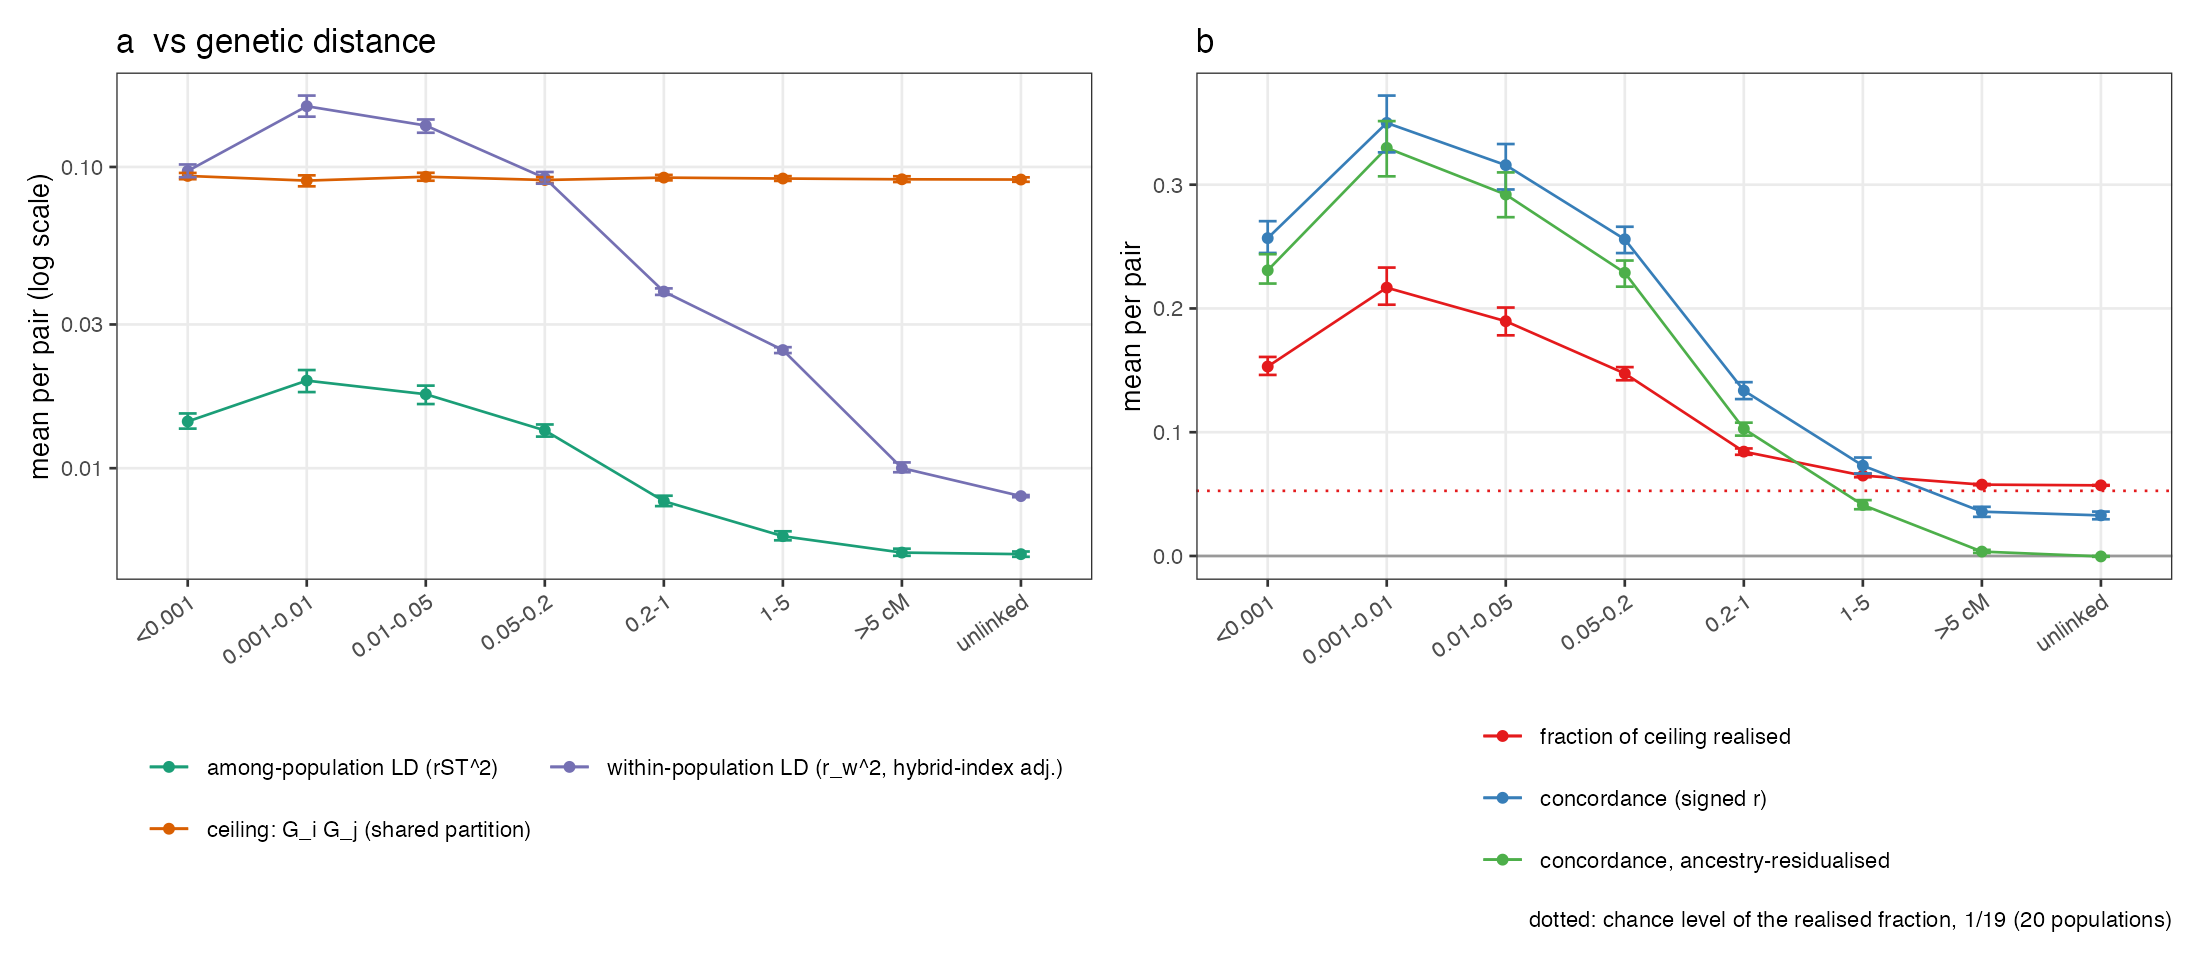
\includegraphics[width=\textwidth]{02_decay_cM.png}
  \caption{As Figure~\ref{fig:decay}, with pairs binned by genetic distance.}
  \label{fig:decay-cm}
\end{figure}

\begin{table}[htbp]
\centering
\scriptsize
\caption{Among- and within-population LD of DI25 unit pairs by physical distance. Means per pair with 95\% chromosome-block bootstrap intervals (2,000 replicates). Ceiling: the among-population LD two loci with their observed $F_{ST}$ would show if they partitioned the populations identically; realised fraction $=\sum r_{ST}^2/\sum G_iG_j$, whose chance level for two unrelated 20-population profiles is $1/19=0.053$. Unlinked: all cross-chromosome pairs.}
\label{tab:decay}
\resizebox{\textwidth}{!}{\begin{tabular}{lccccc}
\toprule
Distance & Ceiling $\overline{G_iG_j}$ & Among-pop.\ LD $\overline{r_{ST}^2}$ & Realised fraction & Concordance (resid.) & Within-pop.\ LD $\overline{r_w^2}$ \\
\midrule
0--5kb & 0.0907 [0.0888, 0.0925] & 0.0220 [0.0213, 0.0227] & 0.2428 [0.2387, 0.2471] & 0.3872 [0.3806, 0.3937] & 0.1828 [0.1788, 0.1866] \\
5--20kb & 0.0904 [0.0887, 0.0923] & 0.0104 [0.0099, 0.0108] & 0.1146 [0.1111, 0.1180] & 0.1755 [0.1687, 0.1822] & 0.0625 [0.0604, 0.0647] \\
20--100kb & 0.0908 [0.0891, 0.0926] & 0.0066 [0.0064, 0.0069] & 0.0726 [0.0708, 0.0747] & 0.0684 [0.0641, 0.0728] & 0.0300 [0.0294, 0.0306] \\
100--500kb & 0.0911 [0.0893, 0.0930] & 0.0056 [0.0054, 0.0058] & 0.0614 [0.0606, 0.0623] & 0.0240 [0.0209, 0.0273] & 0.0206 [0.0202, 0.0210] \\
0.5--2Mb & 0.0909 [0.0892, 0.0928] & 0.0053 [0.0051, 0.0055] & 0.0582 [0.0575, 0.0589] & 0.0050 [0.0024, 0.0080] & 0.0117 [0.0115, 0.0119] \\
2--10Mb & 0.0911 [0.0891, 0.0935] & 0.0052 [0.0051, 0.0054] & 0.0572 [0.0567, 0.0576] & 0.0013 [0.0001, 0.0026] & 0.0083 [0.0081, 0.0084] \\
$>$10Mb & 0.0916 [0.0878, 0.0954] & 0.0052 [0.0050, 0.0054] & 0.0569 [0.0554, 0.0576] & 0.0017 [-0.0039, 0.0053] & 0.0081 [0.0078, 0.0085] \\
unlinked & 0.0908 [0.0893, 0.0924] & 0.0052 [0.0051, 0.0053] & 0.0571 [0.0568, 0.0574] & -0.0004 [-0.0007, -0.0000] & 0.0081 [0.0080, 0.0081] \\
\bottomrule
\end{tabular}}
\end{table}


\FloatBarrier
\subsection{Sorting does not extend to linked neighbours: sorted units are not embedded in sorted haplotypes}

Matching produced controls closely balanced with the 1,577 sorted anchors on \FST, recombination rate, parental differentiation and local unit density (Table~\ref{tab:balance}). If sorting had acted on haplotypes, the neighbours of sorted units should share their population partition over larger distances than the neighbours of equally differentiated unsorted units. The opposite was observed at short range, and no difference at larger distances (Table~\ref{tab:anchors}; Figure~\ref{fig:anchors}). Concordance with neighbours within 5~kb was lower around sorted units than around matched controls (difference $-0.064$ [$-0.085$, $-0.045$]; residualised $-0.062$ [$-0.085$, $-0.042$]), still slightly lower at 5--20~kb ($-0.021$ [$-0.035$, $-0.007$]), and indistinguishable from 20~kb to 2~Mb. Units sorted toward \Fa\ and toward \Fp\ behaved alike.

The pooled within-population LD around sorted units also appeared lower ($-0.078$ within 5~kb), but this difference was almost entirely a dilution artefact: sorted units segregated, on average, in only seven of the 20 populations for which a close neighbour also segregated, versus eleven for controls. Restricted to populations in which both loci segregate, within-population LD around sorted units did not differ from that around controls at any distance (within 5~kb: $-0.013$ [$-0.032$, $0.004$]; 5--20~kb: $0.001$ [$-0.016$, $0.017$]).

Thus, once differentiation is accounted for, the population partition of a sorted locus is shared with its immediate neighbours no more --- and within 20~kb somewhat less --- than that of an unsorted locus, and haplotype-level LD around sorted loci is no stronger. Sorting therefore appears to have acted on individual ancestry-informative alleles rather than carrying extended linked haplotypes with them. The modest short-range concordance deficit suggests that, at sorted loci, the population partition sometimes differs even from that of very close neighbours; whether this reflects fine-scale recombination, gene conversion, or the classification of sorting itself (sorting is defined by near-fixation, which an equally differentiated but unsorted neighbour by definition lacks) has not been resolved.

\begin{figure}[htbp]
  \centering
  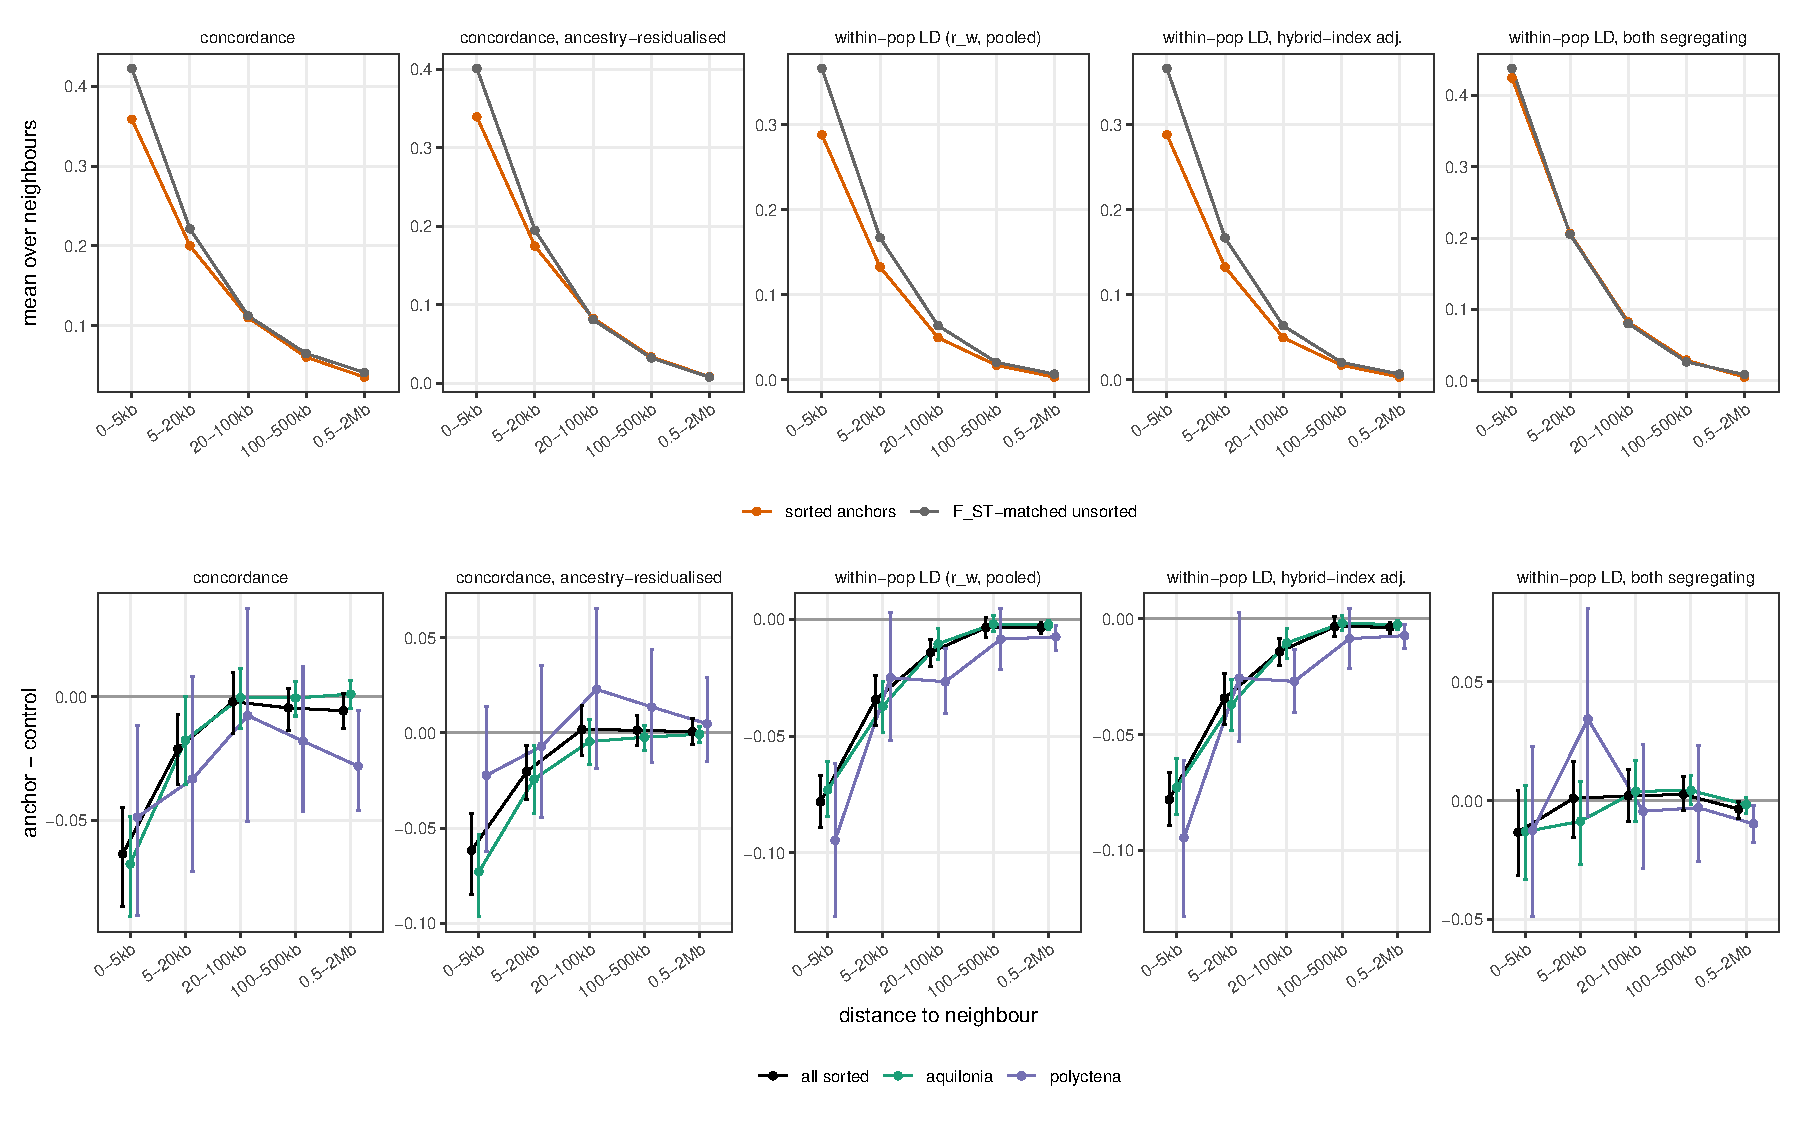
\includegraphics[width=\textwidth]{03_sorted_anchor_decay.pdf}
  \caption{Neighbourhoods of directionally sorted units (anchors) versus \FST-matched unsorted units. Top: means over neighbours by distance. Bottom: anchor $-$ control with 95\% chromosome-block bootstrap intervals, for all anchors and separately for anchors sorted toward \Fa\ and \Fp. The pooled within-population LD panels are diluted for sorted units (see text); Table~\ref{tab:anchors} also reports the version restricted to populations where both loci segregate.}
  \label{fig:anchors}
\end{figure}

\begin{table}[htbp]
\centering
\small
\caption{Covariate balance of the anchor--control matching (means).}
\label{tab:balance}
\begin{tabular}{lcccc}
\toprule
Set & $F_{ST}$ & $\log_{10}$ cM/Mb & Parental differentiation & Units within $\pm$100 kb \\
\midrule
anchors (sorted) & 0.293 & 1.23 & 0.725 & 24.0 \\
matched controls & 0.289 & 1.24 & 0.730 & 24.0 \\
all unsorted & 0.254 & 1.34 & 0.828 & 25.0 \\
\bottomrule
\end{tabular}
\end{table}

\begin{table}[htbp]
\centering
\small
\caption{Neighbourhood concordance and within-population LD around 1577 directionally sorted units (anchors) and $K=5$ unsorted controls per anchor matched on $F_{ST}$, local recombination rate, parental differentiation and local unit density. Difference: anchor $-$ control with 95\% chromosome-block bootstrap interval. Pooled within-population LD is diluted for sorted units, which are monomorphic in most populations; the both-segregating version restricts each pair to populations where both loci segregate.}
\label{tab:anchors}
\begin{tabular}{llccc}
\toprule
Statistic & Distance & Anchors & Controls & Difference [95\% CI] \\
\midrule
Concordance & 0--5kb & 0.359 & 0.423 & -0.064 [-0.085, -0.045] \\
 & 5--20kb & 0.200 & 0.221 & -0.021 [-0.035, -0.007] \\
 & 20--100kb & 0.110 & 0.112 & -0.002 [-0.015, 0.010] \\
 & 100--500kb & 0.060 & 0.065 & -0.005 [-0.014, 0.003] \\
 & 0.5--2Mb & 0.035 & 0.041 & -0.006 [-0.013, 0.001] \\
Concordance (resid.) & 0--5kb & 0.339 & 0.401 & -0.062 [-0.085, -0.042] \\
 & 5--20kb & 0.175 & 0.195 & -0.020 [-0.035, -0.007] \\
 & 20--100kb & 0.083 & 0.081 & 0.002 [-0.012, 0.014] \\
 & 100--500kb & 0.034 & 0.032 & 0.001 [-0.007, 0.009] \\
 & 0.5--2Mb & 0.008 & 0.008 & 0.001 [-0.006, 0.008] \\
Within-pop.\ LD, pooled & 0--5kb & 0.288 & 0.366 & -0.078 [-0.089, -0.067] \\
 & 5--20kb & 0.133 & 0.167 & -0.034 [-0.045, -0.024] \\
 & 20--100kb & 0.049 & 0.063 & -0.014 [-0.020, -0.008] \\
 & 100--500kb & 0.017 & 0.020 & -0.003 [-0.008, 0.001] \\
 & 0.5--2Mb & 0.003 & 0.006 & -0.004 [-0.006, -0.001] \\
Within-pop.\ LD, both segregating & 0--5kb & 0.424 & 0.438 & -0.013 [-0.031, 0.004] \\
 & 5--20kb & 0.206 & 0.205 & 0.001 [-0.016, 0.016] \\
 & 20--100kb & 0.082 & 0.080 & 0.002 [-0.009, 0.013] \\
 & 100--500kb & 0.029 & 0.026 & 0.003 [-0.004, 0.010] \\
 & 0.5--2Mb & 0.005 & 0.009 & -0.004 [-0.007, -0.000] \\
\bottomrule
\end{tabular}
\end{table}


\FloatBarrier
\subsection{Long-range associations between unlinked loci}

Across the 206.8 million cross-chromosome pairs, both tails of residualised concordance and of within-population LD were heavier than under the chromosome-wise permutation null, increasingly so at more extreme thresholds (Table~\ref{tab:longrange}; Figure~\ref{fig:longrange}). At the primary thresholds, the positive tails were inflated 3.0-fold (concordance) and 2.5-fold (within-population LD) relative to the null. The negative tails were inflated by almost exactly the same factors (2.9 and 2.5). An excess of this kind, symmetric in sign, is not what epistatic selection predicts. It is what any structure shared across chromosomes produces, and the permutation removes all such structure, not only pair-specific associations. Among populations, residualisation removed only the main ancestry gradient; additional shared axes of population structure remain, such as the modest, Sielva-dominated axis found in the population-partitioning analyses. Within populations, the equivalent is relatedness among sampled workers. Either generates correlations of both signs between unlinked loci, depending on how each locus loads on the shared axis. Consistent with this, the most connected unit had 23 tail partners for residualised concordance, compared with a 95th percentile of 10 for the most connected unit under the null, as expected if some loci load strongly on a shared axis.

The informative quantity is therefore the asymmetry between the two tails, which shared structure leaves approximately unchanged but which epistasis between compatible ancestries would shift in the positive direction. Raw concordance, which retains the genome-wide ancestry gradient, was strongly asymmetric (0.496 at $T^*=0.8$, versus a null 95\% interval of 0.022--0.083; only the positive tail was inflated), confirming that the test detects a directional, shared signal when one is present. After residualisation, the asymmetry fell within the null interval at nine of ten thresholds between 0.50 and 0.95 (0.067 versus 0.021--0.075 at $T^*$); the exception, at 0.75, exceeded the upper null bound only marginally (0.053 versus 0.047). Within-population LD showed no excess asymmetry at any threshold (0.021 versus 0.002--0.042 at $T^*$). Tail endpoints fell inside BDMI candidate regions at essentially the null rate (residualised concordance 0.266 versus 0.243--0.265; within-population LD 0.264 versus 0.252--0.274).

Thus, beyond what shared population structure and relatedness produce, unlinked loci showed no detectable excess of same-ancestry associations, either among or within populations, and no enrichment of strongly associated loci in BDMI candidate regions. This does not exclude epistatic selection. With 20 populations and 165 individuals, a modest number of incompatible pairs could remain undetected within the tails generated by structure. Moreover, any polygenic incompatibility network resolved in the same direction across populations would load onto the genome-wide ancestry gradient --- which is exactly the component the residualised statistics remove, and which in the raw statistic cannot be distinguished from demographic history. What the results do exclude is a pervasive network of strong, pair-specific associations between unlinked loci of the kind that would make high \FST\ loci jointly differentiated.

\begin{figure}[htbp]
  \centering
  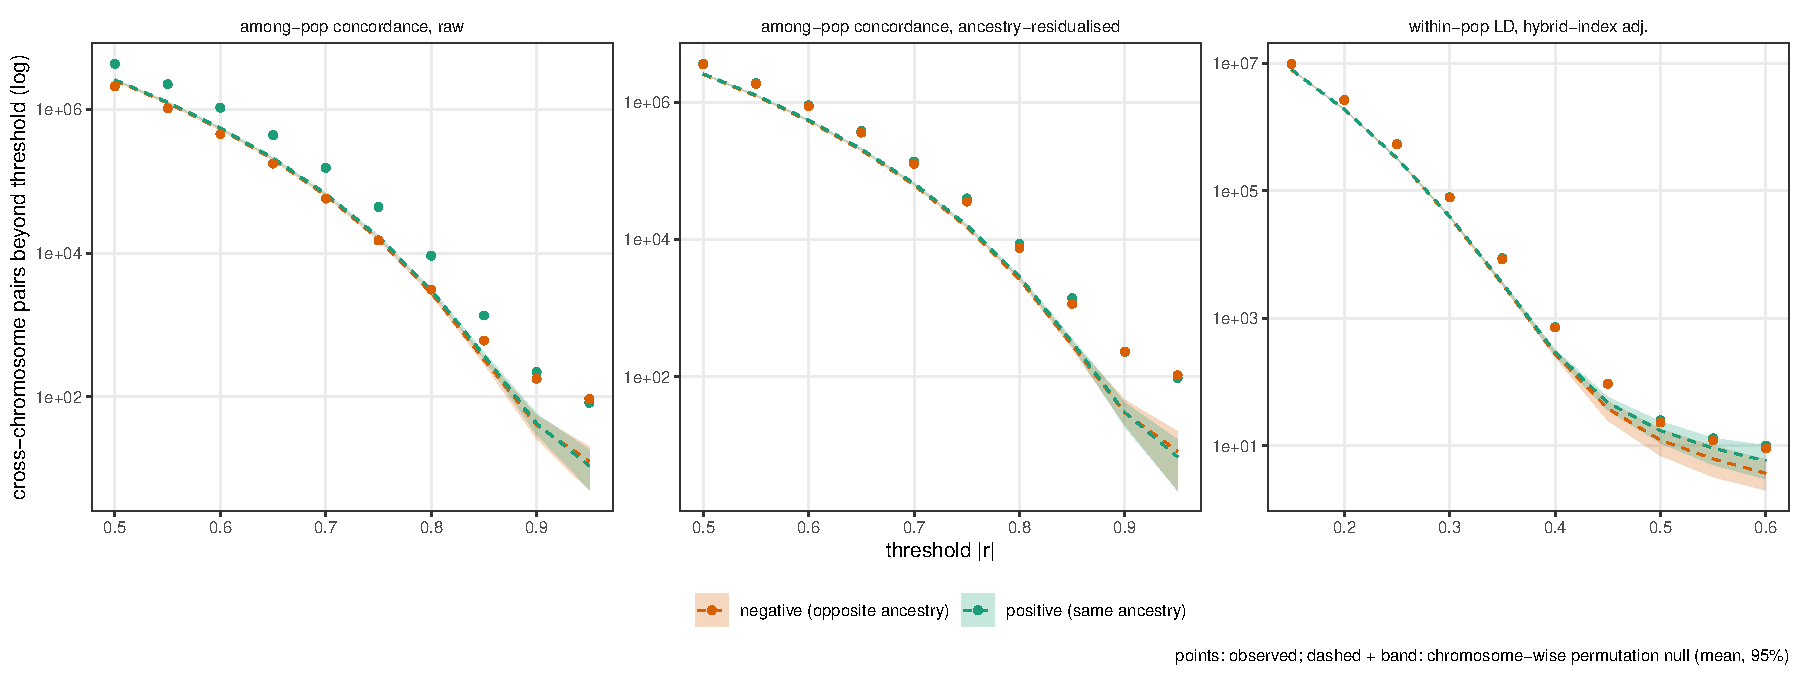
\includegraphics[width=\textwidth]{04_longrange_tail.pdf}
  \caption{Cross-chromosome association tails. Points: observed number of pairs beyond each threshold, separately for the positive (same-ancestry) and negative tails. Dashed lines and bands: mean and 95\% interval of 50 chromosome-wise permutations.}
  \label{fig:longrange}
\end{figure}

\begin{table}[htbp]
\centering
\scriptsize
\caption{Cross-chromosome association tails versus a chromosome-wise permutation null (50 permutations). Positive tail: pairs with $r\geq T^*$ (same parental ancestry at both loci); negative: $r\leq -T^*$; in parentheses, the ratio to the null mean. Asymmetry: $(n_+-n_-)/(n_++n_-)$ with the null 95\% interval. Both tails are inflated by residual population structure (among populations) and kinship (within populations), which the permutation removes; epistasis between compatible ancestries predicts a positive asymmetry beyond the null's. BDMI: fraction of positive-tail endpoints inside BDMI candidate regions (cutoff 13), with the null 95\% interval.}
\label{tab:longrange}
\resizebox{\textwidth}{!}{\begin{tabular}{lcccccc}
\toprule
Statistic & $T^*$ & $+$ tail & $-$ tail & Asymmetry & Null asymmetry & BDMI endpoints [null] \\
\midrule
Among-pop.\ concordance, residualised & 0.80 & 8,621 (3.0$\times$) & 7,532 (2.9$\times$) & 0.067 & [0.021, 0.075] & 0.266 [0.243, 0.265] \\
Among-pop.\ concordance, raw & 0.80 & 9,202 (3.0$\times$) & 3,097 (1.1$\times$) & 0.496 & [0.022, 0.083] & 0.270 [0.244, 0.269] \\
Within-pop.\ LD, hybrid-index adj. & 0.35 & 8,777 (2.5$\times$) & 8,408 (2.5$\times$) & 0.021 & [0.002, 0.042] & 0.264 [0.252, 0.274] \\
\bottomrule
\end{tabular}}
\end{table}


\FloatBarrier
\subsection{Summary}

\begin{itemize}
  \item Among-population LD between ancestry-informative loci realises a quarter of its \FST-determined ceiling at $<5$~kb and falls to chance level beyond $\approx100$~kb, although the ceiling itself is constant with distance. High differentiation and low among-population LD coexist because different loci partition the populations differently.
  \item Within-population LD decays to background over the same distances; individual-level admixture LD is negligible.
  \item Sorted loci do not share their partition with linked neighbours more than equally differentiated unsorted loci do, and within-population LD around them is the same: sorting is allele-specific, not haplotype-wide.
  \item Cross-chromosome association tails are heavier than under a chromosome-wise permutation, but symmetrically in sign, as expected from residual population structure and relatedness. There is no excess of same-ancestry associations between unlinked loci and no enrichment in BDMI candidate regions; a polygenic incompatibility network aligned with the genome-wide ancestry gradient cannot be tested this way.
  \item Whether any of this exceeds neutral expectations: \pending{corrected simulations}.
\end{itemize}


\clearpage
\bibliographystyle{plainnat}
\bibliography{references}

\end{document}
